\documentclass[11pt]{article}

%packages
\usepackage{mathtools}
\usepackage{amsmath}
\usepackage{amssymb}
\usepackage{listings}
\usepackage{xcolor}
\usepackage{graphicx}
\usepackage[margin=1in]{geometry}

%Is this metadata? Title writing info
\title{Enzyme Kinetics in R}
\author{Zane Billings}
\date{}

%Define commands
\newcommand{\np}{\vfill\newpage}
\newcommand{\R}{\texttt{R}}

%Defined colors for xcolor package
\definecolor{cp}{HTML}{592C88} %cp = catamount purple
\definecolor{cg}{HTML}{C1A875} %cg = catamount gold

%Define lstlisting environment appaerance
\lstset{language=R,numbers=left,frame=shadowbox, rulesepcolor=\color{cp}, rulecolor=\color{cg}}

\begin{document}

\maketitle

\section*{Background}
\subsection*{What is Enzyme Kinetics?}
Enzyme kinetics is a subfield of biochemistry which studies the dynamics of chemical reactions which are catalyzed by {\bf enzymes}. Enzymes are a specialized class of protein molecule that have special properties allowing them to speed up biological reactions: this is called the catalytic function of an enzyme.

Enzyme kinetics experiments usually involve taking a known amount of an enzyme, adding it to several different concentrations of its {\bf substrate} (the molecule that the enzyme can interact with), and using an analytical laboratory technique in order to analyze the velocity of the enzyme. Several methods exist for measuring enzyme velocities during a reaction, but the most common are spectrophotometry, radiometry, and fluorescence methods.

\subsection*{Michaelis-Menten Kinetics}
The easiest type of enzymes to describe mathematically are the class of enzymes which are said to follow {\bf Michaelis-Menten kinetics}. Leoner Michaelis and Maud Menten were two biochemists who gave the mathematical model for these enzymes in the beginning of the twentieth century.

In order for an enzyme to fit this model, we must make a few {\bf assumptions}.
\begin{itemize}
	\item All of the enzyme and substrate molecules can diffuse freely (i.e. move wherever they want without constraints) in their container.
	\item The enzyme only binds to one substrate. Enzymes which bind to multiple different substrates (often at the same time) become more complicated and the derivation of their kinematic equations is much more difficult.
	\item The rate of reaction of the enzyme is only affected by two things: intrinsic chemical properties of the enzyme, and the concentration of the substrate. The enzyme can work faster with more substrate, up until the ``saturation point'', where all available enzymes are filled with substrate and the rate of the reaction is capped.
	\item The concentration of the enzyme is much lower than that of the substrate.
\end{itemize}

If we meet all of these conditions, we can describe the rate of the enzyme-substrate reaction with the {\bf Michaelis-Menten Equation}.
\[
V = \frac{V_{\mathrm{max}}[S]}{K_m + [S]}
\]
In the equation, \(V\) is the reaction rate, \(V_{\mathrm{max}}\) is the maximum possible reaction rate, \(K_m\) is the Michaelis-Menten constant, a unique property of every enzyme which describes the concentration of the substrate required for the velocity to reach one half of \(V_{\mathrm{max}}\), and \([S]\) is the concentration of the substrate.

\np

\section*{The Lineweaver-Burk Plot}

Lineweaver and Burk were two biochemists who studied enzyme kinetics and developed a method for using least-squares linear regression to estimate the values of \(K_m\) and \(V_{\mathrm{max}}\) from kinetics data. The LB-plot is also known as a {\bf double-reciprocal plot}. 

Suppose we are testing an enzyme that we will call Hoopsase (almost all enzyme names end with the suffix ``-ase''). We have done a lot of spectrophotometry over the last few days, and we have collected the following data set.

\begin{table}[h!]
\centering
\begin{tabular}{c|c}
	[S], \(\mu\)M & Velocity \(\mu\)Ms\(^{-1}\) \\
	\hline
	2 & 2.9 \\
	3 & 3.8 \\
	4 & 4.4 \\
	5 & 5.0 \\
	6 & 5.4 \\
	7 & 5.8 \\
	8 & 6.2 \\
	9 & 6.4 \\
	10 & 6.7 
\end{tabular}
\caption{Velocity data for various substrate concentrations of the enzyme Hoopsase.}
\label{t:Hoopsase}
\end{table}

You may use the following code snippet to create a data frame with this information in \R. (Change ``ex'' to whatever you want the name to be, of course. I recommend changing the column names as it will be less confusing in the long run.)
\begin{lstlisting}
ex <- data.frame(matrix(c(2,3,4,5,6,7,8,9,10,
                   2.9,3.8,4.4,5.0,5.4,5.8,6.2,6.4,6.7),
                 ncol = 2, byrow = FALSE))
colnames(ex) <- c("S","V")
\end{lstlisting}

The Lineweaver-Burk plot is a graphical method where the reciprocal of the y-data is plotted against the reciprocal of the x-data. Mathematically:
\[
\frac{1}{V} = \frac{K_m + [S]}{V_{\mathrm{max}}[S]} = \frac{K_m}{V_{\mathrm{max}}}\frac{1}{[S]} + \frac{1}{V_{\mathrm{max}}}.
\]

This is an equation of the form \(y=mx+b\), suggesting that if we compute the line of best fit (using a least-squares linear regression method), we can use the slope and intercept of the line to calculate \(K_m\) and \(V_{\mathrm{max}}\) of our enzyme, which gives us a lot of information about how fast the enzyme works.

The Lineweaver-Burk plot was designed originally to be easy to do by hand, but with the power of \R at our disposal, we can do a linear regression model in less than 5 minutes. Let's go through this process step by step on the next page.

\np

\begin{enumerate}

	\item Import the data. The code for doing this is above, underneath Table \ref{t:Hoopsase}. You may also want to use \texttt{plot} (or \texttt{qplot} from the {\it ggplot2} package) to take a quick look at the data.
	\item Take the reciprocals of the data series. You can do this using the \texttt{transform} command if you like that method, but I prefer to declare a new data frame instead.
		\begin{lstlisting}
lb.ex <- data.frame(1/ex$S, 1/ex$V)
colnames(lb.ex) <- c("s.recip,v.recip")
		\end{lstlisting}
	\item Generate the linear regression model using the \texttt{lm} command. You can view almost everything you want to know about the model using the command \texttt{summary}.
	\begin{lstlisting}
model <- lm(
	formula = v.recip~s.recip,
	data = lb.ex)
summary(model)
	\end{lstlisting}
	
	\begin{figure}[h!]
	\centering
	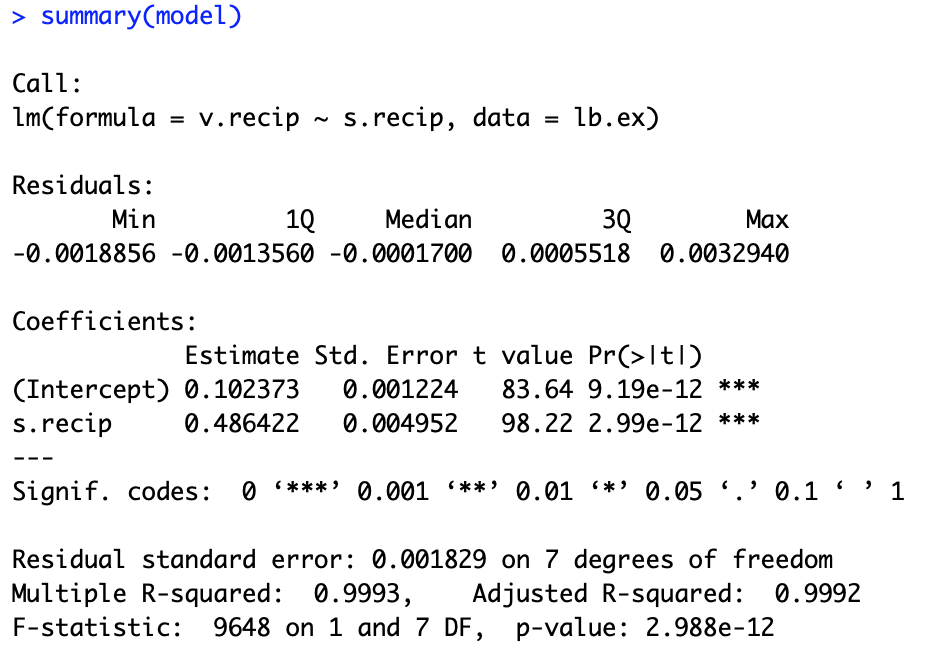
\includegraphics[width=0.5\textwidth]{output_ex_model.png}
	\caption{The output from the summary command. Several relevant outputs are displayed including the parameter estimates and their standard errors, with t-statistics and p-values for each, along with some information about the residuals, \(R^2\) value, and F-test information.}
	\end{figure}
	
	\item In order to judge the goodness-of-fit of the regression line, we can either look at statistics (such as the \(R^2\) value printed above) we can take a qualitative look at a plot of the regression line.
	
	\begin{lstlisting}
	plot(x = lb.ex$s.recip,
     y = lb.ex$v.recipe,
     main = "Lineweaver-Burke Plot",
     xlab = "1/[S]",
     ylab = "1/V")
	abline(model,lty=2)
	\end{lstlisting}
	
	Note that the \texttt{plot} command generates a scatterplot of the data, and the \texttt{abline} command can take our linear model object as an input and create a line based on the model (\texttt{lty=2} species that the line should be a dashed line).
	
	\begin{figure}[ht!]
		\centering
		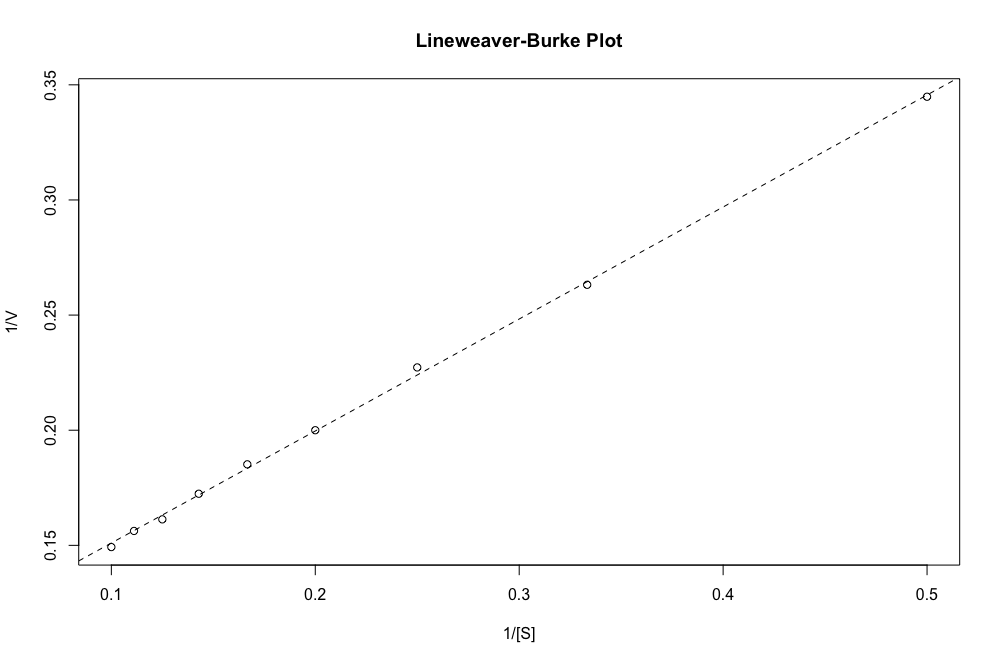
\includegraphics[width=0.75\textwidth]{LB_plot.png}
		\caption{The Lineweaver-Burk plot for the above data.}
		\label{fig:LBexample}
	\end{figure}
	
	\item Now we can use the function \texttt{coef} to extract the slope and the y-intercept values from the linear model object. As we saw from the Lineweaver-Burk equation, we can extract the values of \(K_m\) and \(V_{\mathrm{max}}\) from the parameters of the model. 
	
	\begin{figure}[h!]
		\centering
		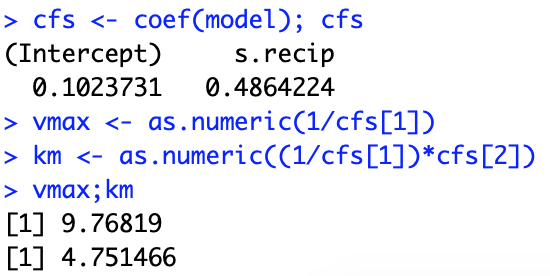
\includegraphics[width=0.5\textwidth]{output_cfs.png}
		\caption{Notice that the \texttt{coef} function returns names with our values (the first value is the y-intercept, and the second value is the slope). Using \texttt{as.numeric()} around our values gets rid of the header part of the data and ensures that our parameter values are stored as numbers only. Look at the Lineweaver-Burk equation and make sure you can explain why we used these formulae in order to get the values of \(K_m\) and \(V_{\mathrm{max}}\).}
		\label{fig:coefout}
	\end{figure}
	
	\item Now we can plot the fitted model against our data. All we need to do is generate a vector of \(\hat{y}\), or predicted, values, and plot it against our original \(x\) values. How do we generate the predicted values? Use the computed values of \(K_m\) and \(V_{\mathrm{max}}\) we just found and plug them into the Michaelis-Menten equation from Page 1.
	
	\np
	
	\begin{lstlisting}
vhat <- (vmax*ex$S)/(km+ex$S)
plot(ex,main = "Lineweaver-Burke Example") +
	lines(x = ex$S, y = vhat,lty=2)
	\end{lstlisting}
	
	\begin{figure}[h!]
	\centering
	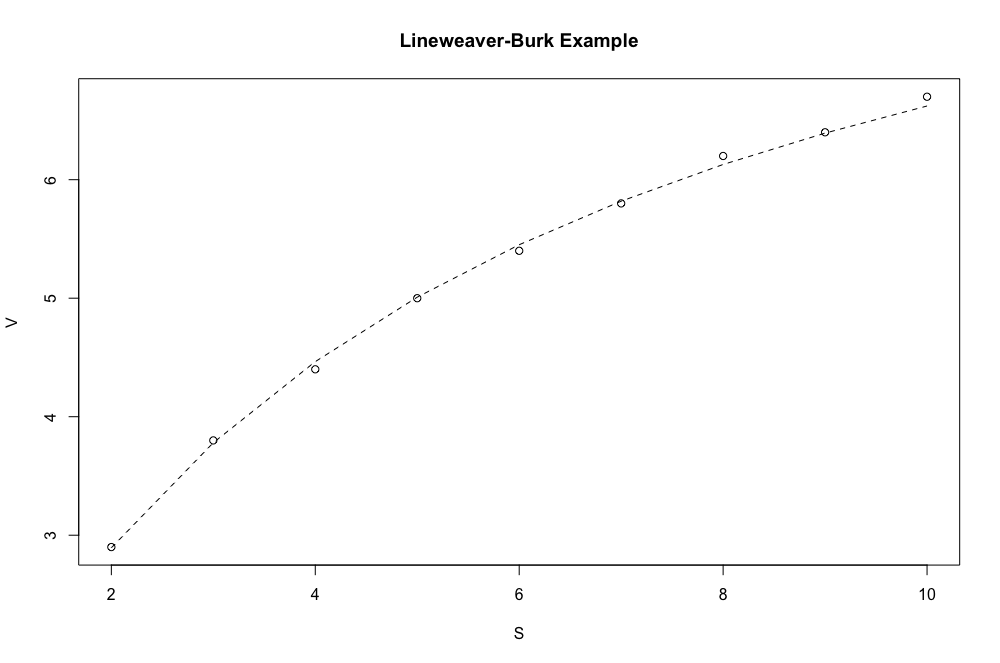
\includegraphics[width=0.75\textwidth]{Ex_Final.png}
	\caption{The Michaelis-Menten plot with our calculated parameter values: it seems to be (qualitatively) a fairly good estimate.}
	\label{Fig:ExFinalPlot}
	\end{figure}		
	
	\item {\bf You try it!} Make sure you can run and understand all of the code needed to do this example. All of the questions in this assignment will use very similar concepts so make sure you understand how this example works!
		
\end{enumerate}

\np

\section*{Analysis of More Realistic Data}
Now that you've seen an example, let's look at some data that might be considered more ``realistic''. Enzyme kinetics data can be hard to collect, and experimental and instrumental error in data collection can lead to some weird data.

{\bf As you complete this assignment, create a TeX document where you include all of your code in a \texttt{listing} file and include all plots you generate in the file as well. Answer all of the questions below. For your final submission, you should submit a compiled .pdf document as well as a .R file containing your R script.}

Now, take a cursory look at the kinetics dataset found on Blackboard. The columns of this dataset are: the substrate concentration [S], and three \(v\) columns...each column represents a new experiment, so we see the experiment was repeated three times.

\begin{enumerate}

\item Import the data file ``kinetics.csv'' which can be found on Blackboard. Rename the columns to make analysis easier. The first thing you need to do is take the average of all three velocity values. (Hint: You can use the following code:
\begin{center}
\begin{verbatim}
kinetics <- transform(kinetics, vave = rowMeans(kinetics[,-1]))
\end{verbatim}
\end{center}

Where ``kinetics" is whatever you want to name your dataframe, and ``vave" is what you want to name your new column.)

For the rest of this analysis, we will only be working with the averages. Make a quick plot of the average velocity vs. [S].

\item Create a Lineweaver-Burk plot for the data, and use \texttt{coef} to look at the slope and y-intercept. Noting that \(K_m\) and \(V_{\mathrm{max}}\) must be {\bf strictly positive} to make any sense, what is wrong with this? Is this model accurate?

\item We can make a second plot called the Hanes-Woolf plot to solve this issue: both sides of the Lineweaver-Burk equation are multiplied by [s], which helps to correct for sampling error in the data. Use the following equation
\[
\frac{[S]}{V} = \frac{1}{V_{\mathrm{max}}}[S] + \frac{K_m}{V_{\mathrm{max}}}
\]
instead of the Lineweaver-Burk equation to create a plot and a linear regression model. Does this model (qualitatively) seem accurate? What are the \(K_m\) and \(V_{\mathrm{max}}\) values you get from this plot? (Use the above equations to figure out how to extract \(K_m\) and \(V_{\mathrm{max}}\) from the output of \texttt{coef}.)

Then, use your estimated parameters in the Michaelis-Menten equation to see how well your predicted values match your true values.

\item Now that you've seen how to use linearization methods to calculate these values, I will let you in on a secret: in the modern computer era, we don't really need (or want) to do any of these methods to estimate parameters. We can instead use an algorithm called {\bf nonlinear least squares} regression. Use the following code:
\begin{center}
\begin{verbatim}
nls.model <- nls(formula = vave ~ Vmax * concentration/(Km + concentration), 
                 data = kinetics,
                 start = list(Km = max(kinetics$vave)/2,
                              Vmax = max(kinetics$vave)))
\end{verbatim}
\end{center}

with ``kinetics'' replaced by the name of your data frame, ``concentration'' replaced by the name of your first data frame column, and ``vave'' replaced by the name of the average velocity column you created in question 1. 

Again, use \texttt{coefs} to extract the parameter values, and make a plot using the Michaelis-Menten equation. Does this model fit the data better than the Hanes-Woolf method?

\item What are some advantages and disadvantages of the linear models (Lineweaver-Burk and Hanes-Woolf)? What about the nonlinear least squares model? (Note that before about the the 90's, nonlinear least squares regression required inaccessible amounts of computing power.)

\item[{\bf BONUS:}] The Eadie-Hofstee diagram is a linearization method similar to Lineweaver-Burk and Hanes-Woolf, but is not often used as it can magnify experimental error. However, if you have very clean data, the Eadie-Hofstee diagram has one major advantage. By simplifying the Eadie-Hofstee equation below, can you determine what this advantage is?
	\begin{equation}
	\frac{V_{\mathrm{max}}}{v}=V_{\mathrm{max}}\left( \frac{K_m+[s]}{V_{\mathrm{max}}[s]} \right)
	\end{equation}


\end{enumerate}


\end{document}